%%%%%%%%%%%%%%%%%%%%%%%%%%%%%%%%%%%%%%%%
% datoteka diploma_predloga.tex
%
% ta verzija sproducira pdf datoteko v pdf/A formatu.
%
% vzorčna datoteka za pisanje diplomskega dela v formatu LaTeX
% na UL Fakulteti za računalništvo in informatiko
%
% Leta 2026 je predlogo posodobil Žiga Emeršič. Predlogo je razdelil na več datotek, uvedel spremenljivke, dodal PDF-A in posodobil navodila (tudi združil določena poglavja in pripravil nova).
% Leta 2021 je predlogo posodobil Franc Solina.
% Leta 2010 je predlogo pripravil Gašper Fijavž.
%
% za upravljanje z literaturo ta vezija uporablja BibLaTeX
%
% svetujemo uporabo Overleaf.com - na tej spletni implementaciji LaTeXa ta vzorec zagotovo pravilno deluje
%
% -------------------------------------------------------------------
% OPOMBA: izvorna vzorčna vsebina predloge (poglavja o LaTeXu, plovkah,
% matematičnem okolju itd.) je bila odstranjena in nadomeščena z vsebino
% diplomske naloge. Vzorec je še vedno dosegljiv v zgodovini repozitorija:
%     git show 156ad49:diploma-predloga.tex
% -------------------------------------------------------------------

% Združljivost s pdfa (sicer nekoliko starejšo različico 1.7)
\DocumentMetadata{pdfstandard = a-2b, pdfversion  = 1.7}

\documentclass[a4paper,12pt,openright]{book}
%\documentclass[a4paper, 12pt, openright, draft]{book}  Nalogo preverite tudi z opcijo draft, ki pokaže, katere vrstice so predolge! Pozor, v draft opciji, se slike ne pokažejo!


%%%%%%%%%%%%%%%%%%%%%%%%%%%%%%%%%%%%%%%%
%  PODATKI O DIPLOMI
%%%%%%%%%%%%%%%%%%%%%%%%%%%%%%%%%%%%%%%%

% Vnesite vaše podatke in podatke mentorjev:
\newcommand{\tauthor}{Tilen Zrnec}
\newcommand{\temail}{tilen.zrnec@student.uni-lj.si}
\newcommand{\tmentor}{izr. prof. dr. Matjaž Kukar}
\newcommand{\tsomentor}{/}

% Odkomentirajte pravi program:
\newcommand{\tstopnja}%
% {VISOKOŠOLSKI STROKOVNI ŠTUDIJSKI PROGRAM\\ PRVE STOPNJE}
{UNIVERZITETNI  ŠTUDIJSKI PROGRAM\\ PRVE STOPNJE\\ RAČUNALNIŠTVO IN INFORMATIKA}
% {INTERDISCIPLINARNI UNIVERZITETNI\\ ŠTUDIJSKI PROGRAM PRVE STOPNJE\\ MULTIMEDIJA}
% {INTERDISCIPLINARNI UNIVERZITETNI\\ ŠTUDIJSKI PROGRAM PRVE STOPNJE\\ UPRAVNA INFORMATIKA}
% {INTERDISCIPLINARNI UNIVERZITETNI\\ ŠTUDIJSKI PROGRAM PRVE STOPNJE\\ RAČUNALNIŠTVO IN MATEMATIKA}

% Odkomentirajte pravo institucijo:
\newcommand{\tinst}%
{Fakulteta za računalništvo in informatiko}
% {Fakulteta za elektrotehniko}
% {Fakulteta za upravo}
% {Fakulteta za matematiko in fiziko}

% Napišite pravo vrsto naloge:
\newcommand{\tvrsta}{Diplomska naloga na univerzitetnem študijskem programu prve stopnje Računalništvo in informatika}

% Opis iz STUDISa:
% TODO: prepiši besedilo teme diplomskega dela iz sistema STUDIS (vnesel ga je mentor).
\newcommand{\tdescription}
{Besedilo teme diplomskega dela študent prepiše iz študijskega informacijskega sistema, kamor ga je vnesel mentor. V nekaj stavkih bo opisal, kaj pričakuje
od kandidatovega diplomskega dela. Kaj so cilji, kakšne metode naj uporabi,
morda bo zapisal tudi ključno literaturo.}
\newcommand{\tdescriptionEn}
{The student shall transcribe the text of the diploma thesis topic from the student information system, where it was entered by the mentor. In a few sentences, they will describe what is expected of the candidate's thesis. What the objectives are, what methods should be used, and perhaps they will also list the key literature.}

% Naslov:
\newcommand{\ttitle}{Tabelarični temeljni modeli}
\newcommand{\ttitleEn}{Tabular Foundation Models}

% Ključne besede:
\newcommand{\tkeywords}{tabelarični temeljni modeli, strojno učenje, tabelarični podatki, ansambli odločitvenih dreves, učenje iz konteksta, OpenML-CC18}
\newcommand{\tkeywordsEn}{tabular foundation models, machine learning, tabular data, decision tree ensembles, in-context learning, OpenML-CC18}

% Zahvala (opcijsko):
% TODO: napiši zahvalo ali celoten ukaz zakomentiraj.
\newcommand{\tzahvala}
{Na tem mestu zapišite, komu se zahvaljujete za pomoč pri izdelavi diplomske naloge oziroma pri vašem študiju nasploh. Pazite, da ne boste koga pozabili. Utegnil vam bo zameriti. Temu se da izogniti tako, da celotno zahvalo izpustite.}

% Posvetilo (opcijsko):
\newcommand{\tposvetilo}
{Svojemu dragemu računalniku.}

%%%%%%%%%%%%%%%%%%%%%%%%%%%%%%%%%%%%%%%%
%  VKLJUČITEV NUJNIH ELEMENTOV 1/2
%%%%%%%%%%%%%%%%%%%%%%%%%%%%%%%%%%%%%%%%

%%%%%%%%%%%%%%%%%%%%%%%%%%%%%%%%%%%%%%%%
% datoteka preambula.tex se uporablja v diploma-FRI-vzorec.tex
%%%%%%%%%%%%%%%%%%%%%%%%%%%%%%%%%%%%%%%%

\usepackage[T1]{fontenc}      % omogoča normalno kopiranje slovenskih črk
\usepackage[utf8]{inputenc}   % omogoča uporabo slovenskih črk kodiranih v formatu UTF-8
\usepackage[slovene,american]{babel}    % naloži, med drugim, slovenske naslove poglavij in delilne vzorce
\usepackage{microtype}         % boljša postavitev
\usepackage[pdftex]{graphicx}  % omogoča vlaganje slik različnih formatov
\usepackage{fancyhdr}          % poskrbi, na primer, za glave strani
\usepackage{amssymb}           % dodatni matematični simboli
\usepackage{amsmath}           % eqref, npr.
\usepackage{amsfonts}
\usepackage[hyphens]{url}
\usepackage{color}
\usepackage{soul}
\usepackage{subcaption}
\usepackage{algorithm}
\usepackage{algpseudocode}
\usepackage[
  backend=biber,
  style=numeric,
  sorting=nty,
]{biblatex}

\addbibresource{literatura.bib}        % pot do literature
\graphicspath{ {./podporno/}{./slike/} } % poti do slik

%%%%%%%%%%%%%%%%%%%%%%%%%%%%%%%%%%%%%%%%
%  enote (decimalna vejica)
%%%%%%%%%%%%%%%%%%%%%%%%%%%%%%%%%%%%%%%%

\usepackage{siunitx}
\sisetup{
  output-decimal-marker = {,}
}

%%%%%%%%%%%%%%%%%%%%%%%%%%%%%%%%%%%%%%%%
%  URLs
%%%%%%%%%%%%%%%%%%%%%%%%%%%%%%%%%%%%%%%%

% najprej podtaknemo opcijo za deljenje URL-jev pri vezajih
\PassOptionsToPackage{hyphens}{url}

% nato naložimo hyperref z vsemi tvojimi nastavitvami
\usepackage[
    pdftex, 
    unicode,                % Podpora za slovenske znake v PDF kazalu/metapodatkih
    colorlinks=true,
    citecolor=black, 
    filecolor=black,
    linkcolor=black, 
    urlcolor=black,
    pdfproducer={LaTeX}, 
    pdfcreator={LaTeX}
]{hyperref}


% \newcommand{\ttitle}{Vzorec diplomskega dela}
% \newcommand{\ttitleEn}{Diploma thesis template}
% \newcommand{\tsubject}{\ttitle}
% \newcommand{\tsubjectEn}{\ttitleEn}
% \newcommand{\tauthor}{Matjaž Kralj}
% \newcommand{\tkeywords}{računalnik, računalnik, računalnik}
% \newcommand{\tkeywordsEn}{computer, computer, computer}

%%%%%%%%%%%%%%%%%%%%%%%%%%%%%%%%%%%%%%%%
%  HYPERREF SETUP
%%%%%%%%%%%%%%%%%%%%%%%%%%%%%%%%%%%%%%%%
\hypersetup{pdftitle={\ttitle}}
\hypersetup{pdfsubject=\ttitleEn}
\hypersetup{pdfauthor={\tauthor}}
\hypersetup{pdfkeywords=\tkeywordsEn}

%%%%%%%%%%%%%%%%%%%%%%%%%%%%%%%%%%%%%%%%
% postavitev strani
%%%%%%%%%%%%%%%%%%%%%%%%%%%%%%%%%%%%%%%%

\addtolength{\marginparwidth}{-20pt} % robovi za tisk
\addtolength{\oddsidemargin}{40pt}
\addtolength{\evensidemargin}{-40pt}

\renewcommand{\baselinestretch}{1.3} % ustrezen razmik med vrsticami
\setlength{\headheight}{15pt}        % potreben prostor na vrhu
\renewcommand{\chaptermark}[1]%
{\markboth{\MakeUppercase{\thechapter.\ #1}}{}} \renewcommand{\sectionmark}[1]%
{\markright{\MakeUppercase{\thesection.\ #1}}} \renewcommand{\headrulewidth}{0.5pt} \renewcommand{\footrulewidth}{0pt}
\fancyhf{}
\fancyhead[LE,RO]{\sl \thepage}
%\fancyhead[LO]{\sl \rightmark} \fancyhead[RE]{\sl \leftmark}
\fancyhead[RE]{\sc \tauthor}              % dodal Solina
\fancyhead[LO]{\sc Diplomska naloga}     % dodal Solina

\newcommand{\BibLaTeX}{{\sc Bib}\LaTeX}
\newcommand{\BibTeX}{{\sc Bib}\TeX}

%%%%%%%%%%%%%%%%%%%%%%%%%%%%%%%%%%%%%%%%
% naslovi
%%%%%%%%%%%%%%%%%%%%%%%%%%%%%%%%%%%%%%%%

\newcommand{\autfont}{\Large}
\newcommand{\titfont}{\LARGE\bf}
\newcommand{\clearemptydoublepage}{\newpage{\pagestyle{empty}\cleardoublepage}}
\setcounter{tocdepth}{1}        % globina kazala

%%%%%%%%%%%%%%%%%%%%%%%%%%%%%%%%%%%%%%%%
% konstrukti
%%%%%%%%%%%%%%%%%%%%%%%%%%%%%%%%%%%%%%%%
\newtheorem{izrek}{Izrek}[chapter]
\newtheorem{trditev}{Trditev}[izrek]
\newenvironment{dokaz}{\emph{Dokaz.}\ }{\hspace{\fill}{$\Box$}}

%%%%%%%%%%%%%%%%%%%%%%%%%%%%%%%%%%%%%%%%
% define medatata
%%%%%%%%%%%%%%%%%%%%%%%%%%%%%%%%%%%%%%%%
\def\Title{\ttitle}
\def\Author{\tauthor, \temail}
\def\Subject{\ttitleEn}
\def\Keywords{\tkeywordsEn}

%%%%%%%%%%%%%%%%%%%%%%%%%%%%%%%%%%%%%%%%
% \convertDate converts D:20080419103507+02'00' to 2008-04-19T10:35:07+02:00
%%%%%%%%%%%%%%%%%%%%%%%%%%%%%%%%%%%%%%%%
\def\convertDate{%
  \getYear
}

{\catcode`\D=12
  \gdef\getYear D:#1#2#3#4{\edef\xYear{#1#2#3#4}\getMonth}
}
\def\getMonth#1#2{\edef\xMonth{#1#2}\getDay}
\def\getDay#1#2{\edef\xDay{#1#2}\getHour}
\def\getHour#1#2{\edef\xHour{#1#2}\getMin}
\def\getMin#1#2{\edef\xMin{#1#2}\getSec}
\def\getSec#1#2{\edef\xSec{#1#2}\getTZh}
\def\getTZh +#1#2{\edef\xTZh{#1#2}\getTZm}
\def\getTZm '#1#2'{%
  \edef\xTZm{#1#2}%
  \edef\convDate{\xYear-\xMonth-\xDay T\xHour:\xMin:\xSec+\xTZh:\xTZm}%
}

%\expandafter\convertDate\pdfcreationdate

%%%%%%%%%%%%%%%%%%%%%%%%%%%%%%%%%%%%%%%%
% get pdftex version string
%%%%%%%%%%%%%%%%%%%%%%%%%%%%%%%%%%%%%%%%
\newcount\countA
\countA=\pdftexversion
\advance \countA by -100
\def\pdftexVersionStr{pdfTeX-1.\the\countA.\pdftexrevision}

%%%%%%%%%%%%%%%%%%%%%%%%%%%%%%%%%%%%%%%%
% XMP data
%%%%%%%%%%%%%%%%%%%%%%%%%%%%%%%%%%%%%%%%
\usepackage{xmpincl}
%\includexmp{pdfa-1b}

%%%%%%%%%%%%%%%%%%%%%%%%%%%%%%%%%%%%%%%%
% pdfInfo
%%%%%%%%%%%%%%%%%%%%%%%%%%%%%%%%%%%%%%%%
\pdfinfo{%
  /Title    (\ttitle)
  /Author   (\tauthor)
  /Subject  (\ttitleEn)
  /Keywords (\tkeywordsEn)
  /ModDate  (\pdfcreationdate)
  /Trapped  /False
}

%%%%%%%%%%%%%%%%%%%%%%%%%%%%%%%%%%%%%%%%
% vključevanje programske kode
%%%%%%%%%%%%%%%%%%%%%%%%%%%%%%%%%%%%%%%%
\usepackage[hypcap=false]{caption}
%\usepackage{minted}
\definecolor{svetlo-siva}{gray}{0.96}
%\usemintedstyle{friendly} % lahko uporabite kakšno drugo temo
%\setminted{
%    fontsize=\footnotesize,
%    baselinestretch=1.1,
%    linenos,            % številčenje vrstic
%    frame=lines,        % črte pred in za
%    framesep=2mm,
%    bgcolor=svetlo-siva, 
%    breaklines=true     % lomljenje dolgih vrstic
%}

% izsek za slovenščino
%\addto\captionsslovene{%
%  \renewcommand{\listingscaption}{Izsek kode}%
%}

% izsek za angleščino
%\addto\captionsenglish{%
%  \renewcommand{\listingscaption}{Code Snippet}%
%}

%%%%%%%%%%%%%%%%%%%%%%%%%%%%%%%%%%%%%%%%
% znaki za copyright stran
%%%%%%%%%%%%%%%%%%%%%%%%%%%%%%%%%%%%%%%%

\newcommand{\CcImageCc}[1]{%
  
\includegraphics[scale=#1]{cc_cc_30.pdf}%
}
\newcommand{\CcImageBy}[1]{%
  
\includegraphics[scale=#1]{cc_by_30.pdf}%
}
\newcommand{\CcImageSa}[1]{%
  
\includegraphics[scale=#1]{cc_sa_30.pdf}%
}

%%%%%%%%%%%%%%%%%%%%%%%%%%%%%%%%%%%%%%%%
\usepackage[autostyle=true]{csquotes} % za narekovaje

% Če želite uporabljati klasične slovenske „narekovaje“ (so enaki nemškim):
\DeclareQuoteAlias{german}{slovene}
% Če pa želite imeti koničaste tipkarske »narekovaje« pa zgornjo vrstico odstranite.


%%%%%%%%%%%%%%%%%%%%%%%%%%%%%%%%%%%%%%%%
%  POMOŽNI UKAZI ZA ČAS PISANJA
%%%%%%%%%%%%%%%%%%%%%%%%%%%%%%%%%%%%%%%%
% Vidna oznaka za nedokončane dele. Pred oddajo morajo iz naloge izginiti
% vsi klici \todo -- poišči jih z:  grep -n "todo{" diploma-predloga.tex
\newcommand{\todo}[1]{%
  \medskip\noindent\fbox{\parbox{0.95\linewidth}{\textbf{TODO:} \textit{#1}}}\medskip%
}

\begin{document}

%%%%%%%%%%%%%%%%%%%%%%%%%%%%%%%%%%%%%%%%
% POVZETEK
%%%%%%%%%%%%%%%%%%%%%%%%%%%%%%%%%%%%%%%%
% Povzetek in abstract pišemo čisto na koncu, ko so znani vsi rezultati.
% Obsegati morata 100-200 besed in vsebovati: (1) stanje področja in problem,
% (2) naš pristop, (3) najpomembnejši rezultat.

\newcommand{\tpovzetek}
{TODO: povzetek napiši na koncu, ko bodo znani vsi rezultati. Obsegati mora med 100 in 200 besed ter zajeti stanje področja in obravnavani problem, naš pristop k njegovemu reševanju ter najpomembnejši rezultat naloge.}

\newcommand{\tabstract}
{TODO: write the abstract last, once all results are known. It must contain between 100 and 200 words and cover the state of the art and the problem addressed, our approach to solving it, and the most important result of the thesis.}

%%%%%%%%%%%%%%%%%%%%%%%%%%%%%%%%%%%%%%%%
%  VKLJUČITEV NUJNIH ELEMENTOV 2/2
%%%%%%%%%%%%%%%%%%%%%%%%%%%%%%%%%%%%%%%%

%%%%%%%%%%%%%%%%%%%%%%%%%%%%%%%%%%%%%%%%
% datoteka naslovnestrani.tex se uporablja v diploma-FRI-vzorec.tex
%%%%%%%%%%%%%%%%%%%%%%%%%%%%%%%%%%%%%%%%

\selectlanguage{slovene}
\frontmatter
\setcounter{page}{1} %
\renewcommand{\thepage}{}       % preprečimo težave s številkami strani v kazalu

%%%%%%%%%%%%%%%%%%%%%%%%%%%%%%%%%%%%%%%%
%naslovnica
\thispagestyle{empty}%
\begin{center}
  {\large\sc Univerza v Ljubljani\\%
    \tinst\\%
  }
  \vskip 10em%
  {\autfont \tauthor\par}%
  {\titfont \ttitle \par}%
  {\vskip 3em \textsc{DIPLOMSKO DELO\\[5mm]         % dodal Solina za ostale študijske programe
         \tstopnja}\par}%
  \vfill\null%
  % izberite pravi habilitacijski naziv mentorja!
  {\large \textsc{Mentor}: \tmentor\par}%
  {\large \textsc{Somentor}:  \tsomentor\par}%
  {\vskip 2em \large Ljubljana, \the\year \par}%
\end{center}
% prazna stran
%\clearemptydoublepage
% izjava o licencah itd. se izpiše na hrbtni strani naslovnice

%%%%%%%%%%%%%%%%%%%%%%%%%%%%%%%%%%%%%%%%
%copyright stran
%%%%%%%%%%%%%%%%%%%%%%%%%%%%%%%%%%%%%%%%
\newpage
\thispagestyle{empty}

\vspace*{5cm}
{\small \noindent
  To delo je ponujeno pod licenco \textit{Creative Commons Priznanje avtorstva-Deljenje pod enakimi pogoji 2.5 Slovenija} (ali novej\v so razli\v cico).
  To pomeni, da se tako besedilo, slike, grafi in druge sestavine dela kot tudi rezultati diplomskega dela lahko prosto distribuirajo,
  reproducirajo, uporabljajo, priobčujejo javnosti in predelujejo, pod pogojem, da se jasno in vidno navede avtorja in naslov tega
  dela in da se v primeru spremembe, preoblikovanja ali uporabe tega dela v svojem delu, lahko distribuira predelava le pod
  licenco, ki je enaka tej.
  Podrobnosti licence so dostopne na spletni strani \href{http://creativecommons.si}{creativecommons.si} ali na Inštitutu za
  intelektualno lastnino, Streliška 1, 1000 Ljubljana.

  \vspace*{1cm}
  \begin{center}% 0.66 / 0.89 = 0.741573033707865
    \CcImageCc{0.741573033707865}\hspace*{1ex}\CcImageBy{1}\hspace*{1ex}\CcImageSa{1}%
  \end{center}
}

\vspace*{1cm}
{\small \noindent
  Izvorna koda diplomskega dela, njeni rezultati in v ta namen razvita programska oprema je ponujena pod licenco GNU General Public License,
  različica 3 (ali novejša). To pomeni, da se lahko prosto distribuira in/ali predeluje pod njenimi pogoji.
  Podrobnosti licence so dostopne na spletni strani \url{http://www.gnu.org/licenses/}.
}

\vfill
\begin{center}
  \ \\ \vfill
  {\em
  Besedilo je oblikovano z urejevalnikom besedil \LaTeX.}
\end{center}

% prazna stran
\clearemptydoublepage

%%%%%%%%%%%%%%%%%%%%%%%%%%%%%%%%%%%%%%%%
% stran 3 med uvodnimi listi
\thispagestyle{empty}
\
\vfill

\bigskip
\noindent\textbf{Kandidat:} \tauthor\\
\noindent\textbf{Naslov:} \ttitle\\
% vstavite ustrezen naziv študijskega programa!
\noindent\textbf{Vrsta naloge:} \tvrsta \\
% izberite pravi habilitacijski naziv mentorja!
\noindent\textbf{Mentor:} \tmentor \\
\noindent\textbf{Somentor:} \tsomentor

\bigskip
\noindent\textbf{Opis:}\\
\tdescription

\bigskip
\noindent\textbf{Title:} \ttitleEn

\bigskip
\noindent\textbf{Description:}\\
\tdescriptionEn

\vfill

\vspace{2cm}

% prazna stran
\clearemptydoublepage

% zahvala
\thispagestyle{empty}\mbox{}\vfill\null\it%
\noindent
\tzahvala
\rm\normalfont

% prazna stran
\clearemptydoublepage

%%%%%%%%%%%%%%%%%%%%%%%%%%%%%%%%%%%%%%%%
% posvetilo, če sama zahvala ne zadošča :-)
\thispagestyle{empty}\mbox{}{\vskip0.20\textheight}\mbox{}\hfill
\begin{minipage}{0.55\textwidth}%
  \tposvetilo
  \normalfont
\end{minipage}

% prazna stran
\clearemptydoublepage

%%%%%%%%%%%%%%%%%%%%%%%%%%%%%%%%%%%%%%%%
% kazalo
\pagestyle{empty}
\def\thepage{}% preprečimo težave s številkami strani v kazalu
\tableofcontents{}

% prazna stran
\clearemptydoublepage

%%%%%%%%%%%%%%%%%%%%%%%%%%%%%%%%%%%%%%%%
% povzetek
\addcontentsline{toc}{chapter}{Povzetek}
\chapter*{Povzetek}

\noindent\textbf{Naslov:} \ttitle
\bigskip

\noindent\textbf{Avtor:} \tauthor
\bigskip

\noindent \tpovzetek

\bigskip

\noindent\textbf{Ključne besede:} \tkeywords.
% prazna stran
\clearemptydoublepage

%%%%%%%%%%%%%%%%%%%%%%%%%%%%%%%%%%%%%%%%
% abstract
\selectlanguage{english}
\addcontentsline{toc}{chapter}{Abstract}
\chapter*{Abstract}

\noindent\textbf{Title:} \ttitleEn
\bigskip

\noindent\textbf{Author:} \tauthor
\bigskip

\noindent \tabstract
\bigskip

\noindent\textbf{Keywords:} \tkeywordsEn.
\selectlanguage{slovene}
% prazna stran
\clearemptydoublepage
\mainmatter
\setcounter{page}{1}
\pagestyle{fancy}

%%%%%%%%%%%%%%%%%%%%%%%%%%%%%%%%%%%%%%%%
% GLAVNA VSEBINA
%%%%%%%%%%%%%%%%%%%%%%%%%%%%%%%%%%%%%%%%

%=========================================================================
\chapter{Uvod}
\label{ch:uvod}
%=========================================================================
% Vsebina poglavja (piši ga med zadnjimi, ko so rezultati znani):
%  - Zakaj so tabelarični podatki pomembni in zakaj so dolgo veljali za
%    področje, kjer globoko učenje zaostaja za ansambli odločitvenih dreves.
%  - Kaj so temeljni modeli in kaj obljubljajo na tabelaričnih podatkih.
%  - Motivacija: ali napovedni model, ki se ga sploh ne uči na ciljni
%    podatkovni množici, prekaša uveljavljene ansamble?
%  - Cilji naloge in raziskovalna vprašanja.
%  - Prispevki naloge.
%  - Zemljevid naloge: kratek opis vsebine po poglavjih (z ukazom \ref,
%    številk poglavij nikoli ne piši ročno).

\todo{Napiši uvod: motivacija, cilji, raziskovalna vprašanja, prispevki in zemljevid naloge.}

%=========================================================================
\chapter{Sorodni pristopi}
\label{ch:sorodni}
%=========================================================================
% Vsebina poglavja:
%  - Klasični pristopi k tabelaričnim podatkom: ansambli odločitvenih dreves
%    kot dolgoletno privzeto orodje.
%  - Globoko učenje na tabelaričnih podatkih in ugotovitve primerjalnih
%    študij, da drevesni modeli pogosto ostajajo boljši.
%  - Temeljni modeli in učenje iz konteksta; prenos ideje na tabelarične
%    podatke (TabPFN, TabICL in sorodni modeli).
%  - Zbirke za primerjalno vrednotenje tabelaričnih modelov (OpenML-CC18,
%    TabArena) in metodološke kritike obstoječih primerjav.
%  - Umestitev: v čem se naša primerjava razlikuje od objavljenih.

\todo{Napiši pregled sorodnih pristopov in umesti nalogo v obstoječi kontekst.}

%=========================================================================
\chapter{Metode in testna metodologija}
\label{ch:metode}
%=========================================================================
% Opis podatkovnih množic ni v tem poglavju, ampak v poglavju \ref{ch:podatki},
% ki prevzema vlogo prvotno načrtovanega podpoglavja 3.1 (Podatkovna nabora).
% To poglavje opisuje algoritme in način testiranja.

\section{Algoritmi}
\label{sec:algoritmi}

V primerjavo smo vključili šest algoritmov za nadzorovano klasifikacijo
tabelaričnih podatkov. Prvi štirje --- naključni gozd, XGBoost, LightGBM in
CatBoost --- so ansambli odločitvenih dreves (angl. \emph{decision tree
ensembles}). Ti že dve desetletji veljajo za privzeto orodje na tabelaričnih
podatkih; primerjalne študije kažejo, da na tipičnih tabelaričnih množicah
srednje velikosti še vedno prekašajo arhitekture globokega učenja, zasnovane
posebej za tabelarične podatke~\cite{grinsztajn2022why}. Zadnja dva, TabPFN in
TabICL, sta tabelarična temeljna modela (angl. \emph{tabular foundation
models}): predhodno naučena modela, ki ciljne podatkovne množice ne vidita med
učenjem, temveč jo ob napovedovanju prejmeta kot kontekst.

Izbor pokriva obe uveljavljeni družini drevesnih ansamblov --- vrečenje
(angl. \emph{bagging}) pri naključnem gozdu in gradientno pospeševanje
(angl. \emph{gradient boosting}) pri preostalih treh --- in znotraj
gradientnega pospeševanja tri implementacije, ki se med seboj razlikujejo po
načinu rasti dreves in po obravnavi kategoričnih atributov. Prav zadnje je za
našo nalogo bistveno, saj se algoritmi zelo razlikujejo po tem, koliko
značilnosti surovih podatkov obravnavajo nativno; to razliko obravnavamo kot
namerno eksperimentalno spremenljivko in jo podrobneje opišemo v
razdelku~\ref{sec:predobdelava}.

Vse algoritme uporabljamo s privzetimi hiperparametri. Edina nastavitev, ki jo
podamo eksplicitno, je naključno seme (\texttt{random\_state=42}); razlogi za
tako zasnovo so navedeni v razdelku~\ref{sec:protokol}. Da so vse druge
nastavitve res privzete in da vsak algoritem prejme le predobdelavo, brez katere
knjižnica podatkov ne sprejme, smo za vseh šest algoritmov preverili s samodejno
revizijo: med učenjem prestrežemo klic knjižnice in njegove parametre primerjamo
s privzetimi, za vsak korak predobdelave pa preverimo, da knjižnica brez njega
podatkov ne sprejme. Od privzetih vrednosti odstopajo le naključno seme ter
nastavitve računanja in izpisovanja, ki modela ne spremenijo.
% Revizija: Diplomsko-delo_Koda/scripts/audit_defaults.py, izpis v
% results/runs/subset_v4_local/diagnostics/audit_defaults.txt.
Ker so pri takem
protokolu privzete vrednosti dejanski del metode, jih pri vsakem algoritmu
posebej navedemo skupaj z virom, iz katerega so povzete. Različice knjižnic so
zbrane v tabeli~\ref{tab:razlicice} in pripete v datoteki
\texttt{requirements.txt} repozitorija s kodo.

% Tabela je generirana iz manifest.json zagona cc18_v3 (scripts/gen_version_table.py
% v repozitoriju s kodo, kopira jo rezultati/generiraj_rezultate.py); zagon cc18_v4
% je tekel v okolju z enakim izpisom pip freeze (skript to preveri).
% Samodejno iz cc18_v3/manifest.json (git 69cc51e, 2026-10-06T15:03:41+00:00). Ne urejaj na roko.
\begin{table}[htbp]
\centering
\caption{Uporabljeni algoritmi, implementacije in pripete različice knjižnic. Pri temeljnih modelih je pod paketom navedena še datoteka z utežmi, saj različica paketa modela ne določa.}
\label{tab:razlicice}
\small
\begin{tabular}{llll}
\hline
Algoritem & Knjižnica & Razred & Različica \\
\hline
Naključni gozd & scikit-learn & \texttt{RandomForestClassifier} & 1.9.1 \\
XGBoost & xgboost & \texttt{XGBClassifier} & 3.4.1 \\
LightGBM & lightgbm & \texttt{LGBMClassifier} & 4.7.0 \\
CatBoost & catboost & \texttt{CatBoostClassifier} & 1.2.10 \\
TabPFN & tabpfn & \texttt{TabPFNClassifier} & 9.1.0 \\
 & \multicolumn{3}{l}{uteži \texttt{tabpfn-v3.5-20260909}} \\
TabICL & tabicl & \texttt{TabICLClassifier} & 2.2.0 \\
 & \multicolumn{3}{l}{uteži \texttt{tabicl-classifier-v2-20260212}} \\
\hline
Python & -- & -- & 3.12.13 \\
PyTorch & torch & -- & 2.14.1+cu130 \\
CUDA & -- & -- & 13.0 \\
\hline
\end{tabular}
\end{table}


\subsection{Naključni gozd}
\label{sec:rf}

Naključni gozd (angl. \emph{random forest}) je ansambel odločitvenih dreves,
naučenih na vzorcih učne množice, dobljenih z vrečenjem~\cite{breiman1996bagging},
pri čemer se v vsakem vozlišču delitev izbira le med naključno podmnožico
atributov; povprečenje napovedi tako razkoreliranih dreves zmanjša varianco
ansambla~\cite{breiman2001random}. Uporabljamo razred
\texttt{RandomForestClassifier} iz knjižnice
scikit-learn~1.9.1~\cite{pedregosa2011scikit} s privzetimi vrednostmi: 100
dreves, gini kot mera nečistosti, neomejena globina in kvadratni koren števila
atributov kot velikost podmnožice kandidatov v vozlišču~\cite{sklearndocsrf}.
Poleg semena podamo \texttt{n\_jobs=-1}, s katerim se drevesa učijo vzporedno.
Naučena drevesa so enaka kot pri zaporednem učenju, vzporedno napovedovanje pa
verjetnosti dreves sešteva v različnem vrstnem redu, zato se ROC-AUC med
ponovljenimi izvedbami lahko razlikuje na četrti ali peti decimalki. Manjkajoče
vrednosti uporabljena različica obravnava sama, kategoričnih atributov pa ne
sprejme, zato jih ordinalno kodiramo; naključni gozd je edini od šestih
algoritmov, ki kategoričnih atributov ne obravnava nativno.
% Vzporedno napovedovanje: na množici cmc pet vzporednih učenj da enaka drevesa,
% deset vzporednih klicev predict_proba pa ne (2026-10-08); največja izmerjena
% razlika ROC-AUC na učenje je 1.3e-4 (blood-transfusion-service-center, 150
% testnih primerov: en drugače urejen izenačen par), sicer do 2.3e-5.
% Manjkajoče vrednosti in kategorije: Diplomsko-delo_Koda/scripts/audit_defaults.py.

\subsection{XGBoost}
\label{sec:xgboost}

Gradientno pospeševanje gradi ansambel zaporedno: vsako novo drevo se prilega
negativnemu gradientu izgube dosedanjega ansambla~\cite{friedman2001greedy}.
XGBoost to zamisel dopolni z aproksimacijo izgube drugega reda, z regularizacijo
kompleksnosti dreves v kriteriju za izbiro delitve in z nativno obravnavo
manjkajočih vrednosti, pri kateri vsako vozlišče iz podatkov določi privzeto
smer za primere z manjkajočo vrednostjo~\cite{chen2016xgboost}. Uporabljamo
razred \texttt{XGBClassifier} iz knjižnice xgboost~3.4.1 s privzetimi
vrednostmi: 100 krogov pospeševanja, stopnja učenja \num{0.3}, največja globina
drevesa 6, koeficient L2 regularizacije 1, brez podvzorčenja primerov in
atributov ter histogramska metoda rasti dreves~\cite{xgboostdocs}. Parameter
\texttt{enable\_categorical} je v tej različici privzeto vklopljen, zato
kategorične atribute podamo kot kategorični podatkovni tip knjižnice pandas in
jih knjižnica obravnava nativno; številske stolpce le pretvorimo v zapis s
plavajočo vejico, saj stolpcev splošnega tipa ne sprejme.
% enable_categorical=True in zavrnitev stolpcev tipa object: preverjeno v nameščeni
% knjižnici xgboost 3.4.1 (Diplomsko-delo_Koda/scripts/audit_defaults.py). Vir
% xgboostdocs se nanaša na različico 2.1.0; navedene privzete vrednosti veljajo tudi v 3.4.1.

\subsection{LightGBM}
\label{sec:lightgbm}

LightGBM je implementacija gradientnega pospeševanja, zasnovana za hitrost na
velikih množicah~\cite{ke2017lightgbm}. Iskanje delitev pospeši z vzorčenjem na
podlagi gradientov (angl. \emph{gradient-based one-side sampling}, GOSS) in z
združevanjem izključujočih se atributov (angl. \emph{exclusive feature
bundling}, EFB), drevesa pa rastejo po listih (angl. \emph{leaf-wise}) namesto
po nivojih, kar daje globlja in bolj asimetrična drevesa kot pri XGBoost.
Uporabljamo razred \texttt{LGBMClassifier} iz knjižnice lightgbm~4.7.0 s
privzetimi vrednostmi: 100 iteracij, stopnja učenja \num{0.1}, 31 listov na
drevo, najmanj 20 primerov v listu in brez podvzorčenja; od obeh tehnik iz
članka je privzeto vklopljeno le združevanje atributov~\cite{lightgbmdocs}.
Poleg semena podamo \texttt{verbosity=-1}, ki izklopi izpisovanje. Manjkajoče
vrednosti in kategorične atribute LightGBM obravnava nativno. Kategorične
atribute mu naštejemo s parametrom \texttt{categorical\_feature}, ker jih
knjižnica, s katero naložimo zbirko OpenML-CC18, označi kot urejene, privzeta
nastavitev LightGBM pa samodejno upošteva le neurejene; rezultat je enak
privzetemu klicu na pravilno označenih atributih.
% Enakost s privzetim klicem: največja razlika napovedanih verjetnosti 0 na
% množicah credit-g in sick (Diplomsko-delo_Koda/scripts/audit_defaults.py).

\subsection{CatBoost}
\label{sec:catboost}

CatBoost je implementacija gradientnega pospeševanja, ki odpravlja premik
napovedi (angl. \emph{prediction shift}) z urejenim pospeševanjem: gradient za
posamezni primer oceni na modelu, naučenem le na primerih pred njim v naključni
permutaciji~\cite{prokhorenkova2018catboost}. Isto zamisel uporabi v urejenih
ciljnih statistikah, s katerimi nativno kodira kategorične atribute, ne da bi
ciljna vrednost primera pronicala v njegov vhod; drevesa so simetrična
(angl. \emph{oblivious}). Uporabljamo razred \texttt{CatBoostClassifier} iz
knjižnice catboost~1.2.10 s privzetimi vrednostmi: 1000 iteracij, globina
drevesa 6, koeficient L2 regularizacije \num{3.0} in samodejno določena stopnja
učenja~\cite{catboostdocs}. Privzetih 1000 iteracij je desetkrat več kot pri
XGBoost in LightGBM, kar upoštevamo pri razlagi časov učenja. Poleg semena
podamo le nastavitvi, ki izklopita izpisovanje in pisanje pomožnih datotek.
Manjkajoče vrednosti v številskih atributih CatBoost obravnava nativno,
kategorične atribute pa mu podamo s parametrom \texttt{cat\_features}, pri čemer
manjkajočo vrednost zapišemo kot niz \texttt{'nan'}, saj je knjižnica v
kategoričnem atributu ne sprejme.

\subsection{TabPFN}
\label{sec:tabpfn}

TabPFN je predstavnik nove družine modelov za tabelarične podatke, ki temelji na
zamisli mreže, prilagojene apriornim podatkom (angl. \emph{prior-data fitted
network}, PFN)~\cite{muller2022transformers}. Namesto da bi se model učil na
ciljni podatkovni množici, ga enkrat in vnaprej naučimo na velikem številu
sintetičnih podatkovnih množic, vzorčenih iz vnaprej določene apriorne
porazdelitve nad nalogami. Naučeni transformer~\cite{vaswani2017attention} se
tako približa Bayesovemu napovedovanju: ob danih označenih primerih vrne
aposteriorno napovedno porazdelitev, ki ustreza apriorni porazdelitvi, na kateri
je bil naučen~\cite{muller2022transformers}.

Posledica je nenavaden potek uporabe: klic metode za učenje ne izvede nobene
posodobitve uteži. Učna množica se skupaj s testnimi primeri poda modelu kot
vhodno zaporedje in napovedi za celotno testno množico nastanejo v enem samem
prehodu naprej. Temu pravimo učenje iz konteksta (angl. \emph{in-context
learning}); ciljna podatkovna množica je za model zgolj vhod, nikoli učni signal.

Prva različica TabPFN~\cite{hollmann2023tabpfn} je to zamisel prenesla na
tabelarične podatke, a z ozkim območjem uporabnosti: do 1000 učnih primerov, do
100 številskih atributov, do 10 razredov in brez manjkajočih vrednosti. Druga
različica~\cite{hollmann2025tabpfn} je model razširila na do \num{10000}
primerov, 500 atributov in 10 razredov ter mu dodala sposobnost, da se z
manjkajočimi vrednostmi, kategoričnimi atributi in osamelci spoprime sam:
avtorji poročajo, da so ga predhodno naučili na približno 100 milijonih
sintetičnih podatkovnih množic, ki take težave vsebujejo, zato se ustreznih
strategij nauči namesto ročno vgrajenih rešitev. Arhitekturno vsaka plast
izvede najprej pozornost po atributih in nato pozornost po
primerih~\cite{hollmann2025tabpfn}.

Tehnično poročilo tretje različice, TabPFN-3, navaja, da je model predhodno
naučen izključno na sintetičnih podatkih, da doseže do \num{1000000} učnih
primerov in 200 atributov ter da na zbirki TabArena en sam prehod naprej z
znatno razliko prekaša vse druge modele, vključno z uglaševanimi in
ansambelskimi primerjalnimi modeli~\cite{grinsztajn2026tabpfn3}.
% PREVERI v poročilu: »200 atributov«? Paket tabpfn 8.5.0 je za TabPFN-3 kot
% uradno podprto mejo navajal 2000 atributov (sporočilo o napaki na CIFAR_10 v
% zagonu cc18_v2).
V naši primerjavi uporabljamo njeno naslednico TabPFN-3.5 iz paketa
tabpfn~9.1.0 (datoteka uteži \texttt{tabpfn-v3.5-20260909}), in sicer z
razredom \texttt{TabPFNClassifier}, privzetimi nastavitvami in podanim
naključnim semenom. Različico modela izberemo izrecno, čeprav je v tem paketu
privzeta, saj je paket privzeto različico med izdajama 8.5.0 in 9.0.0 že
zamenjal (prej je bila privzeta TabPFN-3). Ločenega tehničnega poročila za
TabPFN-3.5 v času pisanja nismo imeli na voljo, zato njegovih lastnosti ne
povzemamo po viru, temveč poročamo le o tistem, kar smo izmerili sami.
\todo{Poišči preverljiv vir za TabPFN-3.5 (tehnično poročilo ali kartica modela) in ga dodaj v literatura.bib.}
Trditve iz poročila za TabPFN-3 navajamo kot kontekst, ne kot ugotovitev te
naloge; ali držijo za njegovo naslednico tudi na zbirki OpenML-CC18 in pod
našim protokolom, je predmet poglavja~\ref{ch:rezultati}, kjer v
razdelku~\ref{sec:rez-zagona} primerjamo tudi obe različici. Pri izvedbi sta
pomembni še dve praktični posebnosti: model za smiselno hitrost potrebuje
grafično procesno enoto in uteži prenese ob prvi uporabi, poleg tega je za prvo
uporabo potreben enkraten sprejem licence prek uporabniškega računa ponudnika,
in sicer za vsako različico modela posebej. Oboje vpliva na
zasnovo izvedbenega okolja in je opisano v razdelku~\ref{sec:okolje}.

\subsection{TabICL}
\label{sec:tabicl}

TabICL izhaja iz iste paradigme kot TabPFN --- gre za predhodno naučen
transformer, ki napoveduje z učenjem iz konteksta --- vendar je arhitekturno
zasnovan tako, da se dobro obnese na večjih podatkovnih
množicah~\cite{qu2025tabicl}. Ključna razlika je dvostopenjska zasnova. V prvi
stopnji model z mehanizmom pozornosti najprej po stolpcih in nato po vrsticah
(angl. \emph{column-then-row attention}) vsako vrstico tabele preslika v
vektorsko predstavitev s fiksno razsežnostjo. Ta predstavitev ni odvisna od
števila atributov, zato se dolžina zaporedja, ki ga obdela druga stopnja, z
večanjem števila atributov ne povečuje. V drugi stopnji transformer za učenje iz
konteksta obdela zaporedje teh vektorskih predstavitev in napove razrede testnih
vrstic.

Avtorji navajajo, da je model predhodno naučen na sintetičnih podatkovnih
množicah z do \num{60000} primeri in da na dostopni strojni opremi obvlada
množice z do \num{500000} primeri. Na 200 klasifikacijskih množicah zbirke
TALENT je po njihovih meritvah primerljiv s TabPFN v2 in do desetkrat hitrejši,
na 53 množicah z več kot \num{10000} primeri pa prekaša tako TabPFN v2 kot
CatBoost~\cite{qu2025tabicl}. V primerjavo smo ga uvrstili kot naravno protiutež
modelu TabPFN: ista paradigma, a drugačna arhitektura, izrecna usmerjenost k
večjim množicam in prosto dostopne uteži.

Uporabljamo razred \texttt{TabICLClassifier} iz paketa tabicl~2.2.0 s privzetimi
nastavitvami in podanim naključnim semenom. Paket privzeto uporabi kontrolno
točko različice TabICLv2 (\texttt{tabicl-classifier-v2-20260212.ckpt}), zato v
resnici vrednotimo to različico~\cite{tabicldocs}; njeno tehnično poročilo kot
glavne izboljšave navaja nov generator sintetičnih podatkov za predhodno učenje,
arhitekturne spremembe in bolje skalirajoč mehanizem
pozornosti~\cite{qu2026tabiclv2}. Enako kot TabPFN tudi TabICL uteži prenese ob
prvi uporabi in za smiselno hitrost potrebuje grafično procesno enoto.

Ker zbirka OpenML-CC18 vsebuje tudi množice, ki po velikosti močno presegajo
razpon, na katerem sta bila oba temeljna modela prvotno predstavljena, ju naš
protokol namerno postavi tudi zunaj njunega najbolj ugodnega območja. Kje se pri
tem ustavita, obravnavamo v poglavju~\ref{ch:rezultati}.

\section{Protokol vrednotenja}
\label{sec:protokol}

\todo{5-fold stratified CV, identical splits, \texttt{random\_state=42}, ROC-AUC binary vs.\ macro-OVR. This is the spine everything else hangs off.}

\section{Politika predobdelave}
\label{sec:predobdelava}

\todo{Your experimental variable. Say explicitly that it's a deliberate design choice, not an oversight, and that it's what Medic3 will finally stress.}

\section{Izvedbeno okolje}
\label{sec:okolje}

\todo{Arnes, H100, SLURM job arrays, micromamba, per-fit checkpointing with atomic \texttt{.partial} files, fail-soft error handling. Fast, descriptive writing. Good warm-up if the algorithms section feels heavy.}

\section{Ponovljivost}
\label{sec:ponovljivost}

\todo{Repo, seeds, pinned versions, PROVENANCE.}

%=========================================================================
\chapter{Materiali}
\label{ch:podatki}
%=========================================================================
% Vsebina poglavja:
%  - Zbirka OpenML-CC18: kako je nastala, kriteriji za uvrstitev množic,
%    zakaj je primerna za to primerjavo (uporabljata jo tudi izvirna članka
%    o modelih TabPFN in TabICL).
%  - Opisna statistika vseh 72 podatkovnih množic: število primerov,
%    število atributov, delež kategoričnih atributov, število razredov,
%    delež manjkajočih vrednosti, uravnoteženost razredov.
%  - Tabela z lastnostmi množic (lahko v prilogo, v besedilu pa povzetek).
%  - Slika: porazdelitev velikosti množic (log-log razsevni diagram
%    število primerov proti številu atributov).
%  - Kje se množice približajo mejam modelov (npr. največje množice).
%
% To poglavje prevzema vlogo prvotno načrtovanega podpoglavja 3.1
% (Podatkovna nabora).

\todo{CC18 half is writable now (inclusion criteria, 72 datasets, size ranges). Leave the Medic3 subsection as a stub until after the Zoom.}

\section{OpenML-CC18}
\label{sec:cc18}

\todo{Kriteriji za uvrstitev podatkovnih množic v zbirko, 72 množic in razponi velikosti: število primerov, število atributov, delež kategoričnih atributov, število razredov in delež manjkajočih vrednosti. Tabela z opisno statistiko in slika porazdelitve velikosti.}

\section{Podatkovni nabor Medic3}
\label{sec:medic3}

\todo{Ostane zgolj okostje do pogovora prek Zooma.}

%=========================================================================
\chapter{Rezultati}
\label{ch:rezultati}
%=========================================================================
% Vsebina poglavja (samo predstavitev meritev, razlaga gre v poglavje 6):
%  - Skupna primerjava: povprečni ROC-AUC in povprečni rang po algoritmih.
%  - Tabela z rezultati po posameznih podatkovnih množicah.
%  - Statistična značilnost razlik med pari algoritmov.
%  - Časovna učinkovitost: čas učenja in čas sklepanja.
%  - Odvisnost uspešnosti od velikosti podatkovne množice in od deleža
%    kategoričnih atributov.
%  - Neuspela učenja in njihovi vzroki.
%  - Popravek predobdelave naključnega gozda in modela XGBoost.
%  - Podatkovni nabor Medic3.

% Vse številke v tem poglavju izvirajo iz repozitorija s kodo
% (Diplomsko-delo_Koda/results/runs; kaj je kateri zagon, pove razdelek
% "Run registry" v njegovem CLAUDE.md). Zbirka OpenML-CC18: sestavljeni nabor
% cc18_v4/combined - naključni gozd in XGBoost iz zagona cc18_v4 (commit 8b601d1,
% po popravku predobdelave), LightGBM, CatBoost, TabPFN-3.5 in TabICL iz glavnega
% zagona cc18_v3 (commit 69cc51e), katerega koda za te štiri algoritme se ni
% spremenila. Nabor Medic3: medic3_raw_v2/combined in medic3_160_v2/combined,
% sestavljena enako. Tabele v mapi rezultati/ in sliki slike/cc18_cd*.pdf
% generira skript rezultati/generiraj_rezultate.py, ki izpiše tudi številke iz
% besedila (vir je naveden v komentarju ob odstavku). Prejšnji zagon cc18_v2
% (TabPFN-3) skript bere iz zgodovine gita, commit 5a14045.
% OPOMBA: angleške izvirnike statističnih izrazov ob prvi pojavitvi prestavi v
% razdelek Protokol vrednotenja, ko bo napisan.

V tem poglavju predstavimo rezultate primerjave šestih algoritmov na
72 podatkovnih množicah zbirke OpenML-CC18~\cite{bischl2021openml} in na
podatkovnem naboru Medic3. Vsak algoritem smo na vsaki podatkovni množici
ovrednotili s petkratnim stratificiranim prečnim preverjanjem (angl.
\emph{stratified cross-validation}), ponovljenim trikrat z različnim mešanjem
primerov. Na vsak par podatkovne množice in algoritma tako pride 15 učenj, na
zbirki OpenML-CC18 skupaj 6480 učenj. Protokol je podrobneje opisan v
razdelku~\ref{sec:protokol}. Model TabPFN smo vrednotili v različici TabPFN-3.5
(razdelek~\ref{sec:tabpfn}), zato ga v tabelah in besedilu tega poglavja
imenujemo s tem imenom. V tem poglavju meritve zgolj
predstavimo, njihovo razlago in omejitve pa obravnavamo v
poglavju~\ref{ch:zakljucek}.

Podatkovno množico imenujemo \emph{nasičena}, če najboljši algoritem na njej
doseže ROC-AUC vsaj \num{0.995}. Takih je 35 od 72 podatkovnih množic. Ker so
razlike med algoritmi na nasičenih množicah blizu zgornje meje metrike, vse
povzetke in statistične teste na zbirki OpenML-CC18 podamo dvakrat: na vseh 72
podatkovnih množicah in na 37 nenasičenih.

\section{Skupna primerjava}
\label{sec:rez-skupno}
% Vir: summary/overall.csv, summary/overall_nonsaturated.csv (cc18_v4/combined)

Tabela~\ref{tab:skupno} povzema uspešnost algoritmov. Za vsako podatkovno
množico algoritme razvrstimo po povprečnem ROC-AUC čez 15 učenj; najboljši
prejme rang 1, izenačeni algoritmi si delijo povprečje rangov, algoritem, ki na
podatkovni množici ni uspel, pa prejme najslabši rang. Povprečni ROC-AUC
računamo le na podatkovnih množicah, na katerih so uspeli vsi algoritmi, da so
povprečja izračunana na isti podmnožici. Na zbirki OpenML-CC18 so vsi algoritmi
uspeli na vseh podatkovnih množicah, zato so povprečja izračunana na vseh.

% Samodejno iz Diplomsko-delo_Koda/results/runs/cc18_v4/combined/summary/overall.csv, results/runs/cc18_v4/combined/summary/overall_nonsaturated.csv (zbirka cc18_v4/combined: naključni gozd in XGBoost iz cc18_v4, commit 8b601d1, ostali iz cc18_v3, commit 69cc51e). Ne urejaj na roko.
\begin{table}[htbp]
\centering
\caption{Skupna primerjava algoritmov na zbirki OpenML-CC18. Vsi algoritmi so uspeli na vseh podatkovnih množicah, zato sta povprečni ROC-AUC in povprečni rang izračunana na vseh 72 oziroma 37 množicah. Zmage štejejo prvo mesto, vključno z izenačitvami.}
\label{tab:skupno}
\footnotesize
\setlength{\tabcolsep}{4pt}
\begin{tabular}{lrrrrrrr}
\hline
 & \multicolumn{4}{c}{vseh 72 množic} & \multicolumn{3}{c}{37 nenasičenih množic} \\
Algoritem & ROC-AUC & rang & zmage & neuspehi & ROC-AUC & rang & zmage \\
\hline
TabPFN-3.5 & \num{0.9416} & \num{1.42} & 48 & 0 & \num{0.8877} & \num{1.24} & 29 \\
TabICL & \num{0.9391} & \num{1.86} & 26 & 0 & \num{0.8836} & \num{2.03} & 8 \\
CatBoost & \num{0.9283} & \num{3.39} & 1 & 0 & \num{0.8657} & \num{3.32} & 0 \\
LightGBM & \num{0.9222} & \num{4.47} & 0 & 0 & \num{0.8552} & \num{4.49} & 0 \\
XGBoost & \num{0.9208} & \num{4.67} & 1 & 0 & \num{0.8516} & \num{4.97} & 0 \\
Naključni gozd & \num{0.9184} & \num{5.19} & 0 & 0 & \num{0.8511} & \num{4.95} & 0 \\
\hline
\end{tabular}
\end{table}


Najnižji povprečni rang doseže TabPFN-3.5 (\num{1.42}), ki je bil najboljši na
48 podatkovnih množicah, sledi mu TabICL (\num{1.86}, 26 zmag). Med drevesnimi
ansambli je najuspešnejši CatBoost s povprečnim rangom \num{3.39}, sledijo mu
LightGBM (\num{4.47}), XGBoost (\num{4.67}) in naključni gozd (\num{5.19}). Enak
vrstni red se pokaže v povprečnem ROC-AUC, ki se giblje od \num{0.9416} pri
TabPFN-3.5 do \num{0.9184} pri naključnem gozdu. Brez nasičenih podatkovnih
množic se razlike v povprečnem ROC-AUC povečajo: TabPFN-3.5 doseže \num{0.8877},
CatBoost \num{0.8657} in naključni gozd \num{0.8511}. Vrstni red po povprečnem
rangu ostane enak z eno izjemo: na nenasičenih podatkovnih množicah je naključni
gozd (\num{4.95}) pred modelom XGBoost (\num{4.97}), čeprav ima XGBoost višji
povprečni ROC-AUC (\num{0.8516} proti \num{0.8511}).

\section{Statistična značilnost razlik}
\label{sec:rez-znacilnost}
% Vir: summary/friedman.csv, summary/nemenyi.csv, summary/wilcoxon_holm.csv
% in njihove različice *_nonsaturated.csv (cc18_v4/combined)

Razlike med algoritmi smo preverili po postopku za primerjavo več
klasifikatorjev na več podatkovnih množicah, ki ga
priporoča Demšar~\cite{demsar2006statistical}: s Friedmanovim testom, ki
preveri ničelno domnevo, da so vsi algoritmi enakovredni, z Nemenyijevim testom
kot naknadnim testom (angl. \emph{post-hoc test}) nad povprečnimi rangi ter s
parnimi Wilcoxonovimi testi predznačenih rangov (angl. \emph{Wilcoxon
signed-rank test}) s Holmovim popravkom za večkratno primerjanje. Stopnja
značilnosti je povsod $\alpha = 0{,}05$.

O zavrnitvi ničelne domneve Friedmanovega testa odločimo na podlagi statistike
$F_F$, ki sta jo predlagala Iman in Davenport in jo Demšar priporoča namesto
preveč konservativne statistike $\chi^2_F$~\cite{demsar2006statistical}.
Friedmanov test ničelno domnevo zavrne tako na vseh 72 podatkovnih množicah
($\chi^2_F = \num{251.30}$, $F_F = \num{164.15}$ s $(5, 355)$ prostostnimi
stopnjami, $p = \num{5.1e-90}$) kot na 37 nenasičenih ($\chi^2_F =
\num{132.43}$, $F_F = \num{90.68}$ s $(5, 180)$ prostostnimi stopnjami, $p =
\num{2.7e-47}$). Kritična razdalja
(angl. \emph{critical difference}) Nemenyijevega testa znaša \num{0.889} na vseh
in \num{1.240} na nenasičenih podatkovnih množicah; povprečna ranga dveh
algoritmov, ki se razlikujeta za manj od kritične razdalje, se značilno ne
razlikujeta. Rezultat prikazujeta diagrama kritične razdalje na
sliki~\ref{fig:cd}.

\begin{figure}[htbp]
\centering
\begin{subfigure}{\linewidth}
\centering
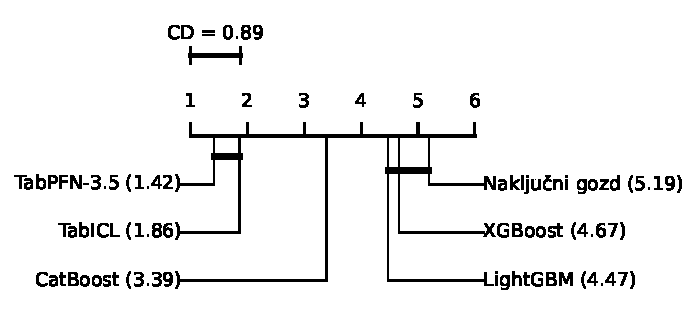
\includegraphics[width=\linewidth]{cc18_cd.pdf}
\caption{Vseh 72 podatkovnih množic.}
\label{fig:cd-vse}
\end{subfigure}

\medskip
\begin{subfigure}{\linewidth}
\centering
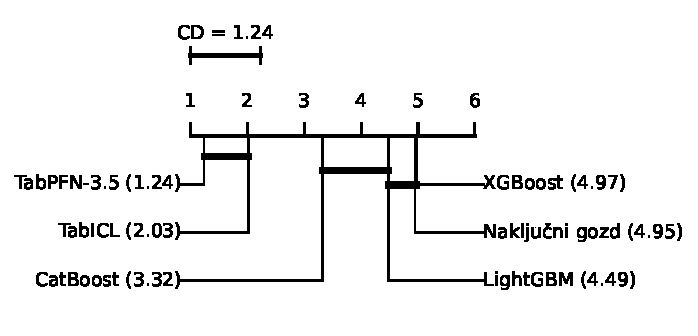
\includegraphics[width=\linewidth]{cc18_cd_nenasicene.pdf}
\caption{37 nenasičenih podatkovnih množic.}
\label{fig:cd-nenasicene}
\end{subfigure}
\caption{Diagrama kritične razdalje (Nemenyijev test, $\alpha = 0{,}05$). Na osi
so povprečni rangi, daljica CD nad osjo ponazarja kritično razdaljo, odebeljene
vodoravne črte pa povezujejo skupine algoritmov, med katerimi razlika ni
značilna.}
\label{fig:cd}
\end{figure}

Na vseh podatkovnih množicah Nemenyijev test loči tri skupine. Temeljna modela
TabPFN-3.5 in TabICL se med seboj značilno ne razlikujeta (razlika povprečnih
rangov \num{0.44}), sta pa značilno boljša od vseh drevesnih ansamblov. CatBoost
se značilno razlikuje od vseh preostalih algoritmov, LightGBM, XGBoost in
naključni gozd pa tvorijo skupino brez značilnih razlik. Na nenasičenih
podatkovnih množicah se zaradi večje kritične razdalje v skupino brez značilne
razlike združita tudi CatBoost in LightGBM (razlika povprečnih rangov
\num{1.16}).

% Samodejno iz Diplomsko-delo_Koda/results/runs/cc18_v4/combined/summary/wilcoxon_holm.csv, results/runs/cc18_v4/combined/summary/wilcoxon_holm_nonsaturated.csv (zbirka cc18_v4/combined: naključni gozd in XGBoost iz cc18_v4, commit 8b601d1, ostali iz cc18_v3, commit 69cc51e). Ne urejaj na roko.
\begin{table}[htbp]
\centering
\caption{Parni Wilcoxonovi testi predznačenih rangov s Holmovim popravkom. Razlika je povprečna razlika ROC-AUC (prvi minus drugi algoritem) čez podatkovne množice, na katerih sta uspela oba; zmage so število množic, na katerih je boljši prvi oziroma drugi. Z zvezdico so označene razlike, značilne pri $\alpha = 0{,}05$.}
\label{tab:wilcoxon}
\footnotesize
\setlength{\tabcolsep}{2.5pt}
\begin{tabular}{lrrlrrl}
\hline
 & \multicolumn{3}{c}{vseh 72 množic} & \multicolumn{3}{c}{37 nenasičenih množic} \\
Par algoritmov & razlika & zmage & $p_\mathrm{Holm}$ & razlika & zmage & $p_\mathrm{Holm}$ \\
\hline
TabPFN-3.5 -- TabICL & \num{0.0025} & 45:23 & \num{0.0018}$^{*}$ & \num{0.0041} & 29:8 & \num{0.0026}$^{*}$ \\
TabPFN-3.5 -- CatBoost & \num{0.0133} & 69:3 & \num{1.5e-11}$^{*}$ & \num{0.0220} & 36:1 & \num{3.5e-10}$^{*}$ \\
TabPFN-3.5 -- LightGBM & \num{0.0194} & 71:1 & \num{2.5e-12}$^{*}$ & \num{0.0325} & 37:0 & \num{2.2e-10}$^{*}$ \\
TabPFN-3.5 -- XGBoost & \num{0.0209} & 71:1 & \num{2.5e-12}$^{*}$ & \num{0.0361} & 37:0 & \num{2.2e-10}$^{*}$ \\
TabPFN-3.5 -- Naključni gozd & \num{0.0232} & 72:0 & \num{2.5e-12}$^{*}$ & \num{0.0366} & 37:0 & \num{2.2e-10}$^{*}$ \\
TabICL -- CatBoost & \num{0.0109} & 66:6 & \num{4.0e-10}$^{*}$ & \num{0.0179} & 34:3 & \num{7.5e-08}$^{*}$ \\
TabICL -- LightGBM & \num{0.0170} & 69:3 & \num{3.1e-11}$^{*}$ & \num{0.0284} & 35:2 & \num{9.2e-09}$^{*}$ \\
TabICL -- XGBoost & \num{0.0184} & 69:3 & \num{1.5e-11}$^{*}$ & \num{0.0321} & 35:2 & \num{2.0e-09}$^{*}$ \\
TabICL -- Naključni gozd & \num{0.0208} & 69:3 & \num{1.5e-11}$^{*}$ & \num{0.0325} & 35:2 & \num{1.6e-09}$^{*}$ \\
CatBoost -- LightGBM & \num{0.0061} & 58:14 & \num{4.0e-07}$^{*}$ & \num{0.0105} & 29:8 & \num{4.9e-05}$^{*}$ \\
CatBoost -- XGBoost & \num{0.0075} & 56:16 & \num{9.6e-07}$^{*}$ & \num{0.0142} & 33:4 & \num{1.9e-06}$^{*}$ \\
CatBoost -- Naključni gozd & \num{0.0099} & 65:7 & \num{3.7e-08}$^{*}$ & \num{0.0146} & 33:4 & \num{4.9e-05}$^{*}$ \\
LightGBM -- XGBoost & \num{0.0014} & 41:31 & \num{0.2349} & \num{0.0037} & 24:13 & \num{0.0262}$^{*}$ \\
LightGBM -- Naključni gozd & \num{0.0038} & 51:21 & \num{0.0570} & \num{0.0041} & 22:15 & \num{0.6468} \\
XGBoost -- Naključni gozd & \num{0.0024} & 45:27 & \num{0.2349} & \num{0.0004} & 19:18 & \num{0.6468} \\
\hline
\end{tabular}
\end{table}


Parni Wilcoxonovi testi v tabeli~\ref{tab:wilcoxon} potrdijo razlike med
temeljnima modeloma in vsemi drevesnimi ansambli ter med CatBoostom in
preostalimi tremi ansambli, tudi na nenasičenih podatkovnih množicah. Med
LightGBM, modelom XGBoost in naključnim gozdom na vseh podatkovnih množicah
noben par ni značilen (najmanjši $p_\mathrm{Holm} = \num{0.0570}$ pri paru
LightGBM--naključni gozd). Na nenasičenih množicah je LightGBM značilno boljši od
modela XGBoost ($p_\mathrm{Holm} = \num{0.0262}$), para z naključnim gozdom pa
ostaneta neznačilna. Parni test tako pokaže značilno razliko pri nekaterih
parih, pri katerih je Nemenyijev test ne: na vseh podatkovnih množicah pri paru
TabPFN-3.5--TabICL ($p_\mathrm{Holm} = \num{0.0018}$), na nenasičenih pa pri
parih TabPFN-3.5--TabICL ($p_\mathrm{Holm} = \num{0.0026}$), CatBoost--LightGBM
($p_\mathrm{Holm} = \num{4.9e-5}$) in LightGBM--XGBoost. TabPFN-3.5 je od TabICL
na vseh podatkovnih množicah boljši na 45 in slabši na 23, povprečna razlika
ROC-AUC pa znaša zgolj \num{0.0025}.

\section{Rezultati po podatkovnih množicah}
\label{sec:rez-mnozice}
% Vir: summary/pivot.csv, summary/ranks.csv (cc18_v4/combined); razlike so
% izračunane iz vrednosti v tabeli \ref{tab:mnozice}.

Povprečni ROC-AUC vseh algoritmov na posameznih podatkovnih množicah je zbran v
tabeli~\ref{tab:mnozice}. Najvišji ROC-AUC je drevesni ansambel dosegel le na
dveh podatkovnih množicah, obe pa sta nasičeni: na množici tic-tac-toe je
CatBoost (\num{1.0000}) presegel TabICL (\num{0.9996}), na množici
wall-robot-navigation pa je XGBoost najboljši temeljni model presegel za manj kot
\num{0.0001}. Na preostalih 70 podatkovnih množicah je najboljši temeljni model
presegel najboljši drevesni ansambel, na množicah MiceProtein in
banknote-authentication za manj kot \num{0.0001}. Največja razlika v prid
temeljnih modelov je na množicah GesturePhaseSegmentationProcessed
(\num{0.0767}), madelon (\num{0.0499}), balance-scale (\num{0.0489}), vehicle
(\num{0.0478}) in cylinder-bands (\num{0.0476}).

Razlike med temeljnima modeloma so praviloma majhne: mediana absolutne razlike
ROC-AUC med TabPFN-3.5 in TabICL čez podatkovne množice je \num{0.0011}.
Največji razliki v prid TabPFN-3.5 sta na množicah cylinder-bands
(\num{0.0322}) in Bioresponse (\num{0.0232}), v prid TabICL pa na množicah
climate-model-simulation-crashes (\num{0.0111}) in analcatdata\_dmft
(\num{0.0072}).

% Samodejno iz Diplomsko-delo_Koda/results/runs/cc18_v4/combined/summary/pivot.csv (zbirka cc18_v4/combined: naključni gozd in XGBoost iz cc18_v4, commit 8b601d1, ostali iz cc18_v3, commit 69cc51e). Ne urejaj na roko.
{\scriptsize
\setlength{\tabcolsep}{3pt}
\begin{longtable}{>{\raggedright\arraybackslash}p{3.3cm}rrrrrr}
\caption{Povprečni ROC-AUC po podatkovnih množicah (povprečje čez 15 učenj). Nakl.\ gozd označuje naključni gozd. Najboljša vrednost v vrstici je v krepkem tisku (primerjava na štiri decimalke), zvezdica pa označuje nasičeno podatkovno množico (najboljši ROC-AUC vsaj \num{0.995}).}
\label{tab:mnozice} \\
\hline
Podatkovna množica & TabPFN-3.5 & TabICL & CatBoost & LightGBM & XGBoost & Nakl.\ gozd \\
\hline
\endfirsthead
\hline
Podatkovna množica & TabPFN-3.5 & TabICL & CatBoost & LightGBM & XGBoost & Nakl.\ gozd \\
\hline
\endhead
\hline
\endfoot
adult & \textbf{\num{0.9342}} & \num{0.9262} & \num{0.9302} & \num{0.9294} & \num{0.9265} & \num{0.9067} \\
analcatdata\_\allowbreak authorship$^{*}$ & \textbf{\num{1.0000}} & \textbf{\num{1.0000}} & \num{0.9997} & \num{0.9998} & \num{0.9995} & \num{0.9999} \\
analcatdata\_\allowbreak dmft & \num{0.5815} & \textbf{\num{0.5887}} & \num{0.5536} & \num{0.5605} & \num{0.5438} & \num{0.5385} \\
balance-scale$^{*}$ & \textbf{\num{0.9996}} & \num{0.9993} & \num{0.9506} & \num{0.9279} & \num{0.9318} & \num{0.8387} \\
bank-marketing & \textbf{\num{0.9466}} & \num{0.9419} & \num{0.9380} & \num{0.9364} & \num{0.9317} & \num{0.9269} \\
banknote-authentication$^{*}$ & \textbf{\num{1.0000}} & \textbf{\num{1.0000}} & \textbf{\num{1.0000}} & \num{0.9996} & \num{0.9999} & \num{0.9999} \\
Bioresponse & \textbf{\num{0.8854}} & \num{0.8622} & \num{0.8732} & \num{0.8736} & \num{0.8715} & \num{0.8713} \\
blood-transfusion-service-center & \num{0.7557} & \textbf{\num{0.7587}} & \num{0.7361} & \num{0.6982} & \num{0.6816} & \num{0.6861} \\
breast-w$^{*}$ & \textbf{\num{0.9951}} & \num{0.9949} & \num{0.9931} & \num{0.9926} & \num{0.9902} & \num{0.9924} \\
car$^{*}$ & \textbf{\num{1.0000}} & \num{0.9999} & \num{0.9997} & \num{0.9992} & \num{0.9998} & \num{0.9987} \\
churn & \textbf{\num{0.9343}} & \num{0.9316} & \num{0.9240} & \num{0.9189} & \num{0.9208} & \num{0.9166} \\
CIFAR\_\allowbreak 10 & \textbf{\num{0.9158}} & \num{0.9050} & \num{0.9104} & \num{0.8949} & \num{0.8981} & \num{0.8508} \\
climate-model-simulation-crashes & \num{0.9527} & \textbf{\num{0.9639}} & \num{0.9562} & \num{0.9423} & \num{0.9446} & \num{0.9195} \\
cmc & \textbf{\num{0.7518}} & \num{0.7516} & \num{0.7250} & \num{0.7081} & \num{0.7003} & \num{0.7014} \\
cnae-9$^{*}$ & \num{0.9977} & \textbf{\num{0.9982}} & \num{0.9952} & \num{0.9809} & \num{0.9932} & \num{0.9943} \\
connect-4 & \textbf{\num{0.9564}} & \num{0.9424} & \num{0.9196} & \num{0.9133} & \num{0.9249} & \num{0.8912} \\
credit-approval & \num{0.9401} & \textbf{\num{0.9404}} & \num{0.9361} & \num{0.9319} & \num{0.9271} & \num{0.9331} \\
credit-g & \textbf{\num{0.8022}} & \num{0.7947} & \num{0.7882} & \num{0.7700} & \num{0.7610} & \num{0.7811} \\
cylinder-bands & \textbf{\num{0.9447}} & \num{0.9125} & \num{0.8727} & \num{0.8807} & \num{0.8854} & \num{0.8971} \\
Devnagari-Script$^{*}$ & \textbf{\num{0.9999}} & \textbf{\num{0.9999}} & \num{0.9994} & \num{0.9981} & \num{0.9983} & \num{0.9962} \\
diabetes & \textbf{\num{0.8428}} & \num{0.8405} & \num{0.8335} & \num{0.8001} & \num{0.7916} & \num{0.8253} \\
dna$^{*}$ & \num{0.9954} & \textbf{\num{0.9956}} & \num{0.9946} & \num{0.9946} & \num{0.9947} & \num{0.9932} \\
dresses-sales & \textbf{\num{0.6327}} & \num{0.6259} & \num{0.6045} & \num{0.5679} & \num{0.5686} & \num{0.5735} \\
electricity$^{*}$ & \textbf{\num{0.9968}} & \num{0.9804} & \num{0.9562} & \num{0.9545} & \num{0.9731} & \num{0.9702} \\
eucalyptus & \textbf{\num{0.9387}} & \num{0.9374} & \num{0.9147} & \num{0.9088} & \num{0.9015} & \num{0.9136} \\
Fashion-MNIST$^{*}$ & \textbf{\num{0.9951}} & \textbf{\num{0.9951}} & \num{0.9932} & \num{0.9934} & \num{0.9935} & \num{0.9907} \\
first-order-theorem-proving & \textbf{\num{0.8641}} & \num{0.8627} & \num{0.8439} & \num{0.8416} & \num{0.8413} & \num{0.8379} \\
Gesture\allowbreak Phase\allowbreak Segmentation\allowbreak Processed & \textbf{\num{0.9749}} & \num{0.9617} & \num{0.8983} & \num{0.8890} & \num{0.8927} & \num{0.8922} \\
har$^{*}$ & \textbf{\num{1.0000}} & \textbf{\num{1.0000}} & \num{0.9999} & \num{0.9999} & \num{0.9999} & \num{0.9995} \\
ilpd & \num{0.7807} & \textbf{\num{0.7878}} & \num{0.7564} & \num{0.7490} & \num{0.7353} & \num{0.7497} \\
Internet-Advertisements & \textbf{\num{0.9914}} & \num{0.9837} & \num{0.9758} & \num{0.9809} & \num{0.9785} & \num{0.9847} \\
isolet$^{*}$ & \textbf{\num{0.9997}} & \textbf{\num{0.9997}} & \num{0.9993} & \num{0.9990} & \num{0.9988} & \num{0.9984} \\
jm1 & \textbf{\num{0.7913}} & \num{0.7803} & \num{0.7459} & \num{0.7426} & \num{0.7229} & \num{0.7484} \\
jungle\_\allowbreak chess\_\allowbreak 2pcs\_\allowbreak raw\_\allowbreak endgame\_\allowbreak complete$^{*}$ & \textbf{\num{0.9970}} & \num{0.9872} & \num{0.9754} & \num{0.9747} & \num{0.9779} & \num{0.9385} \\
kc1 & \textbf{\num{0.8583}} & \num{0.8570} & \num{0.8266} & \num{0.7807} & \num{0.7881} & \num{0.8245} \\
kc2 & \num{0.8430} & \textbf{\num{0.8442}} & \num{0.8236} & \num{0.7841} & \num{0.7681} & \num{0.8184} \\
kr-vs-kp$^{*}$ & \textbf{\num{0.9998}} & \textbf{\num{0.9998}} & \num{0.9995} & \num{0.9997} & \num{0.9997} & \num{0.9988} \\
letter$^{*}$ & \textbf{\num{1.0000}} & \textbf{\num{1.0000}} & \num{0.9997} & \num{0.9997} & \num{0.9996} & \num{0.9995} \\
madelon & \textbf{\num{0.9745}} & \num{0.9706} & \num{0.9246} & \num{0.8947} & \num{0.8838} & \num{0.7786} \\
mfeat-factors$^{*}$ & \textbf{\num{0.9999}} & \textbf{\num{0.9999}} & \num{0.9990} & \num{0.9987} & \num{0.9983} & \num{0.9979} \\
mfeat-fourier & \textbf{\num{0.9941}} & \num{0.9937} & \num{0.9840} & \num{0.9816} & \num{0.9817} & \num{0.9812} \\
mfeat-karhunen$^{*}$ & \textbf{\num{0.9998}} & \textbf{\num{0.9999}} & \num{0.9991} & \num{0.9983} & \num{0.9976} & \num{0.9973} \\
mfeat-morphological & \textbf{\num{0.9715}} & \num{0.9704} & \num{0.9638} & \num{0.9566} & \num{0.9580} & \num{0.9554} \\
mfeat-pixel$^{*}$ & \textbf{\num{0.9998}} & \textbf{\num{0.9998}} & \num{0.9994} & \num{0.9990} & \num{0.9988} & \num{0.9987} \\
mfeat-zernike & \num{0.9908} & \textbf{\num{0.9919}} & \num{0.9745} & \num{0.9661} & \num{0.9676} & \num{0.9680} \\
Mice\allowbreak Protein$^{*}$ & \textbf{\num{1.0000}} & \textbf{\num{1.0000}} & \textbf{\num{1.0000}} & \textbf{\num{1.0000}} & \num{0.9997} & \num{0.9999} \\
mnist\_\allowbreak 784$^{*}$ & \textbf{\num{0.9999}} & \textbf{\num{0.9999}} & \num{0.9993} & \num{0.9995} & \num{0.9996} & \num{0.9990} \\
nomao$^{*}$ & \textbf{\num{0.9979}} & \num{0.9967} & \num{0.9954} & \num{0.9950} & \num{0.9957} & \num{0.9942} \\
numerai28.6 & \textbf{\num{0.5379}} & \num{0.5312} & \num{0.5196} & \num{0.5228} & \num{0.5137} & \num{0.5137} \\
optdigits$^{*}$ & \textbf{\num{1.0000}} & \textbf{\num{1.0000}} & \num{0.9998} & \num{0.9996} & \num{0.9995} & \num{0.9996} \\
ozone-level-8hr & \textbf{\num{0.9435}} & \num{0.9404} & \num{0.9263} & \num{0.9200} & \num{0.9213} & \num{0.9099} \\
pc1 & \textbf{\num{0.8955}} & \num{0.8929} & \num{0.8759} & \num{0.8576} & \num{0.8463} & \num{0.8461} \\
pc3 & \textbf{\num{0.8728}} & \num{0.8706} & \num{0.8433} & \num{0.8208} & \num{0.8146} & \num{0.8377} \\
pc4 & \textbf{\num{0.9647}} & \num{0.9610} & \num{0.9524} & \num{0.9454} & \num{0.9445} & \num{0.9427} \\
pendigits$^{*}$ & \textbf{\num{0.9999}} & \textbf{\num{0.9999}} & \num{0.9998} & \num{0.9997} & \num{0.9997} & \num{0.9997} \\
Phishing\allowbreak Websites$^{*}$ & \num{0.9981} & \textbf{\num{0.9983}} & \num{0.9954} & \num{0.9959} & \num{0.9966} & \num{0.9956} \\
phoneme & \textbf{\num{0.9784}} & \num{0.9759} & \num{0.9535} & \num{0.9535} & \num{0.9552} & \num{0.9616} \\
qsar-biodeg & \num{0.9451} & \textbf{\num{0.9478}} & \num{0.9371} & \num{0.9360} & \num{0.9313} & \num{0.9340} \\
satimage$^{*}$ & \textbf{\num{0.9964}} & \num{0.9958} & \num{0.9917} & \num{0.9911} & \num{0.9908} & \num{0.9897} \\
segment$^{*}$ & \textbf{\num{0.9978}} & \num{0.9977} & \num{0.9957} & \num{0.9952} & \num{0.9947} & \num{0.9952} \\
semeion$^{*}$ & \num{0.9992} & \textbf{\num{0.9993}} & \num{0.9978} & \num{0.9968} & \num{0.9956} & \num{0.9961} \\
sick$^{*}$ & \textbf{\num{0.9989}} & \num{0.9979} & \num{0.9981} & \num{0.9977} & \num{0.9971} & \num{0.9968} \\
spambase & \textbf{\num{0.9930}} & \num{0.9924} & \num{0.9883} & \num{0.9894} & \num{0.9879} & \num{0.9864} \\
splice$^{*}$ & \num{0.9960} & \textbf{\num{0.9964}} & \num{0.9949} & \num{0.9946} & \num{0.9957} & \num{0.9923} \\
steel-plates-fault & \textbf{\num{0.9801}} & \num{0.9760} & \num{0.9661} & \num{0.9666} & \num{0.9655} & \num{0.9606} \\
texture$^{*}$ & \textbf{\num{1.0000}} & \textbf{\num{1.0000}} & \num{0.9999} & \num{0.9998} & \num{0.9998} & \num{0.9996} \\
tic-tac-toe$^{*}$ & \num{0.9992} & \num{0.9996} & \textbf{\num{1.0000}} & \num{0.9992} & \num{0.9991} & \num{0.9961} \\
vehicle & \textbf{\num{0.9834}} & \num{0.9782} & \num{0.9356} & \num{0.9301} & \num{0.9300} & \num{0.9274} \\
vowel$^{*}$ & \textbf{\num{1.0000}} & \textbf{\num{1.0000}} & \num{0.9992} & \num{0.9970} & \num{0.9965} & \num{0.9989} \\
wall-robot-navigation$^{*}$ & \num{0.9999} & \num{0.9999} & \textbf{\num{1.0000}} & \textbf{\num{1.0000}} & \textbf{\num{1.0000}} & \num{0.9999} \\
wdbc$^{*}$ & \num{0.9970} & \textbf{\num{0.9973}} & \num{0.9937} & \num{0.9926} & \num{0.9935} & \num{0.9895} \\
wilt$^{*}$ & \num{0.9958} & \textbf{\num{0.9960}} & \num{0.9915} & \num{0.9885} & \num{0.9891} & \num{0.9868} \\
\end{longtable}
}


\section{Časovna zahtevnost}
\label{sec:rez-casi}
% Vir: summary/overall.csv (mediane in vsote časov), results.csv (stolpca device
% in hostname), oboje cc18_v4/combined

Čase učenja in napovedovanja povzema tabela~\ref{tab:casi}. Pri branju je treba
upoštevati, da so drevesni ansambli tekli na osmih procesorskih jedrih,
temeljna modela pa na grafični procesni enoti NVIDIA H100 v dveh izvedbah
(stolpec \texttt{device} v datoteki z rezultati), zato izmerjeni časi
primerjajo kombinacijo algoritma in strojne opreme. Učenja so tekla na
različnih vozliščih gruče, zato časi med algoritmi in med podatkovnimi
množicami niso strogo primerljivi. Pri temeljnih modelih klic učenja ne
posodobi uteži (razdelek~\ref{sec:tabpfn}), zato večji del njune računske
zahtevnosti odpade na napovedovanje.

% Samodejno iz Diplomsko-delo_Koda/results/runs/cc18_v4/combined/summary/overall.csv, results/runs/cc18_v4/combined/results.csv (zbirka cc18_v4/combined: naključni gozd in XGBoost iz cc18_v4, commit 8b601d1, ostali iz cc18_v3, commit 69cc51e). Ne urejaj na roko.
\begin{table}[htbp]
\centering
\caption{Časovna zahtevnost algoritmov. Mediani sta izračunani čez vseh 1080 učenj posameznega algoritma, skupni čas je vsota časa učenja in napovedovanja čez vsa učenja. Časi niso neposredno primerljivi med algoritmi, ki so tekli na različni strojni opremi; temeljna modela sta tekla na dveh izvedbah grafične procesne enote (H100 80GB HBM3 in H100 PCIe), drevesni ansambli pa na procesorjih različnih vozlišč gruče.}
\label{tab:casi}
\footnotesize
\begin{tabular}{llrrr}
\hline
 & & \multicolumn{2}{c}{mediana na učenje [s]} & skupni čas \\
Algoritem & naprava & učenje & napovedovanje & [h] \\
\hline
CatBoost & CPU (8 jeder) & \num{4.584} & \num{0.0043} & \num{47.8} \\
XGBoost & CPU (8 jeder) & \num{0.176} & \num{0.0037} & \num{5.3} \\
TabICL & GPU (H100) & \num{0.487} & \num{0.2000} & \num{4.0} \\
LightGBM & CPU (8 jeder) & \num{0.252} & \num{0.0057} & \num{2.5} \\
TabPFN-3.5 & GPU (H100) & \num{0.211} & \num{0.4870} & \num{2.5} \\
Naključni gozd & CPU (8 jeder) & \num{0.121} & \num{0.0151} & \num{0.3} \\
\hline
\end{tabular}
\end{table}


Skupni čas vseh 6480 učenj je znašal \num{62.3} ure, od tega \num{47.8} ure
CatBoost. Njegova mediana časa učenja (\num{4.584} s) je od 18- do 38-krat
večja od median preostalih treh drevesnih ansamblov (od \num{0.121} do
\num{0.252} s), kar je skladno z njegovim privzetim številom iteracij
(razdelek~\ref{sec:catboost}). Mediani časa učenja temeljnih modelov sta
\num{0.211} s (TabPFN-3.5) in \num{0.487} s (TabICL), mediani časa
napovedovanja pa \num{0.487} s in \num{0.200} s, medtem ko drevesni ansambli
napovedujejo v največ \num{0.015} s.

\section{Neuspela in pomnilniško zahtevna učenja}
\label{sec:rez-pomnilnik}
% Vir: results.csv (stolpci error, raw_error), summary/pivot.csv (CIFAR_10),
% results/runs/cc18_v3/PROVENANCE.md in sacct.txt (MaxRSS, dodeljeni pomnilnik,
% ponovna oddaja opravila 20176087).

Vseh 6480 učenj je uspelo. Oba temeljna modela sta na vseh podatkovnih množicah
sprejela surove podatke, zato minimalni popravek iz politike predobdelave
(razdelek~\ref{sec:predobdelava}) ni bil uporabljen nikjer.

Računsko najzahtevnejša je bila podatkovna množica CIFAR\_10 s 3072 atributi.
TabPFN-3.5 jo je sprejel, čeprav je predhodna različica na njej zaradi števila
atributov odpovedala (razdelek~\ref{sec:rez-zagona}), in na njej dosegel
najvišji povprečni ROC-AUC (\num{0.9158}, pred CatBoostom s \num{0.9104}).
TabICL je na tej množici porabil do 394~GiB delovnega pomnilnika (največja
velikost rezidentnega pomnilnika, ki jo je zabeležil razporejevalnik opravil).
Prvi poskus z dodeljenimi 240~GiB je razporejevalnik zato prekinil; TabICL je
uspel šele na vozlišču z več pomnilnika in z dodeljenimi 480~GiB, kjer je
dosegel povprečni ROC-AUC \num{0.9050}.

\section{Primerjava z modelom TabPFN-3}
\label{sec:rez-zagona}
% Vir: izpis skripta generiraj_rezultate.py (zagon cc18_v3 proti cc18_v2 iz gita,
% commit 5a14045: results.csv, summary/overall.csv, summary/wilcoxon_holm.csv;
% sporočilo o napaki TabPFN-3 na CIFAR_10 je v stolpcu error zagona cc18_v2).
% TabICL in TabPFN-3.5 v končnih rezultatih sta iz cc18_v3, zato je primerjava
% teh dveh modelov s cc18_v2 neposredna.

Protokol smo izvedli tudi s prejšnjo zamrznitvijo različic knjižnic, v kateri je
bil namesto modela TabPFN-3.5 uporabljen TabPFN-3 (paket tabpfn~8.5.0).
TabPFN-3.5 je imel višji povprečni ROC-AUC kot TabPFN-3 na 56 od 71 podatkovnih
množic, na katerih sta uspela oba (mediana razlike \num{0.0007}). Največje
izboljšanje je na množicah cylinder-bands (\num{0.0357}) in connect-4
(\num{0.0164}), največje poslabšanje pa na množicah
climate-model-simulation-crashes (\num{-0.0038}) in
blood-transfusion-service-center (\num{-0.0035}). TabPFN-3 je poleg tega
zavrnil množico CIFAR\_10, ker število atributov presega uradno podprtih 2000;
omejitev je sicer mogoče izklopiti z nastavitvijo
\texttt{ignore\_pretraining\_limits=True}, ki je zaradi protokola s privzetimi
nastavitvami nismo uporabili.

Sprememba modela je zamenjala vrstni red temeljnih modelov. S TabPFN-3 je bil
prvi TabICL (povprečni rang \num{1.58}, 49 zmag) pred modelom TabPFN-3
(\num{1.90}, 22 zmag), parni Wilcoxonov test pa je pokazal, da je TabICL
značilno boljši (boljši na 47 in slabši na 20 podatkovnih množicah,
$p_\mathrm{Holm} = \num{0.0046}$). S TabPFN-3.5 je razmerje obrnjeno
(razdelek~\ref{sec:rez-znacilnost}). Rezultati modela TabICL, katerega paket se
med zamrznitvama ni spremenil, so ostali skoraj enaki: ROC-AUC se razlikuje na
147 od 1065 učenj, ki so uspela pri obeh zamrznitvah, največ za \num{0.0037}.

\section{Odvisnost od lastnosti podatkovnih množic}
\label{sec:rez-lastnosti}

\todo{Odvisnost prednosti temeljnih modelov od števila primerov, števila atributov, števila razredov in deleža kategoričnih atributov. Pred pisanjem dodaj v repozitorij s kodo skript, ki to izračuna (npr. Spearmanov koeficient in razbitje po velikosti), da bo imela vsaka številka generiran vir.}

\section{Podatkovni nabor Medic3}
\label{sec:rez-medic3}
% Vir: tab_medic3.tex, tab_medic3_test.tex in izpis skripta
% generiraj_rezultate.py (medic3_raw_v2/combined, medic3_160_v2/combined;
% primerjava z medic3_raw in medic3_160 pred popravkom). Diagnostika LightGBM:
% medic3_raw/diagnostics in medic3_160/diagnostics, datoteke
% lightgbm_4.7.0_independent.csv in lightgbm_4.6.0_independent.csv, ki jih
% ustvari scripts/diagnose_lightgbm_medic3.py (prva delitev, seme 42).

Na podatkovnem naboru Medic3 (razdelek~\ref{sec:medic3}) smo vseh šest
algoritmov ovrednotili v dveh različicah: z vsemi 220 razredi (\num{122093}
primerov in 275 atributov) in s 160 najpogostejšimi razredi (\num{117825}
primerov). Druga različica obstaja zato, ker TabPFN-3.5 sprejme največ 160
razredov; primere preostalih razredov smo zavrgli. Protokol je enak kot na
zbirki OpenML-CC18, torej 15 učenj na algoritem in različico. Rezultate povzema
tabela~\ref{tab:medic3}.

% Samodejno iz Diplomsko-delo_Koda/results/runs/medic3_raw_v2/combined/summary/per_dataset.csv, results/runs/medic3_160_v2/combined/summary/per_dataset.csv (naključni gozd in XGBoost iz medic3_raw_v2/medic3_160_v2, ostali iz medic3_raw/medic3_160). Ne urejaj na roko.
\begin{table}[htbp]
\centering
\caption{Rezultati na podatkovnem naboru Medic3 z vsemi 220 razredi in s 160 najpogostejšimi razredi: povprečni ROC-AUC $\pm$ standardni odklon čez 15 učenj ter mediani časa učenja in napovedovanja na učenje. -- označuje neuspeh vseh učenj (TabPFN-3.5 sprejme največ 160 razredov). Časi primerjajo kombinacijo algoritma in strojne opreme (razdelek~\ref{sec:rez-casi}).}
\label{tab:medic3}
\footnotesize
\setlength{\tabcolsep}{3pt}
\begin{tabular}{lrrrrrr}
\hline
 & \multicolumn{3}{c}{220 razredov} & \multicolumn{3}{c}{160 razredov} \\
 & & \multicolumn{2}{c}{mediana [s]} & & \multicolumn{2}{c}{mediana [s]} \\
Algoritem & ROC-AUC & učenje & napoved. & ROC-AUC & učenje & napoved. \\
\hline
TabPFN-3.5 & \multicolumn{1}{c}{--} & -- & -- & \num{0.9614} $\pm$ \num{0.0007} & \num{2.3} & \num{74.4} \\
CatBoost & \num{0.9551} $\pm$ \num{0.0010} & \num{8142.6} & \num{0.3} & \num{0.9599} $\pm$ \num{0.0009} & \num{5549.8} & \num{0.2} \\
TabICL & \num{0.9499} $\pm$ \num{0.0016} & \num{10.3} & \num{79.8} & \num{0.9543} $\pm$ \num{0.0011} & \num{10.0} & \num{76.6} \\
XGBoost & \num{0.9306} $\pm$ \num{0.0023} & \num{303.5} & \num{3.9} & \num{0.9400} $\pm$ \num{0.0019} & \num{129.6} & \num{1.8} \\
Naključni gozd & \num{0.8394} $\pm$ \num{0.0025} & \num{13.6} & \num{0.5} & \num{0.8726} $\pm$ \num{0.0014} & \num{11.1} & \num{0.3} \\
LightGBM & \num{0.5028} $\pm$ \num{0.0048} & \num{59.8} & \num{1.2} & \num{0.5057} $\pm$ \num{0.0063} & \num{49.7} & \num{1.3} \\
\hline
\end{tabular}
\end{table}


Na različici z vsemi 220 razredi TabPFN-3.5 ni uspel v nobenem od 15 učenj:
knjižnica je učenje zavrnila s sporočilom, da število razredov presega uradno
podprtih 160. Najvišji povprečni ROC-AUC je dosegel CatBoost (\num{0.9551}),
sledijo mu TabICL (\num{0.9499}), XGBoost (\num{0.9306}), naključni gozd
(\num{0.8394}) in LightGBM (\num{0.5028}). Na različici s 160 razredi je bil
najboljši TabPFN-3.5 (\num{0.9614}), tesno pred CatBoostom (\num{0.9599}),
sledijo TabICL (\num{0.9543}), XGBoost (\num{0.9400}), naključni gozd
(\num{0.8726}) in LightGBM (\num{0.5057}). Standardni odklon čez 15 učenj je
pri vseh algoritmih največ \num{0.0063}.

Ker gre za en sam podatkovni nabor, testov za primerjavo na več podatkovnih
množicah ne moremo uporabiti~\cite{demsar2006statistical}. Pare algoritmov smo
zato primerjali s popravljenim t-testom za ponovljeno prečno
preverjanje~\cite{bouckaert2004evaluating}, ki pri oceni variance razlik
upošteva, da se učni deli zaporednih učenj prekrivajo~\cite{nadeau2003inference}.
Statistika $t = \bar{d} \,/\, \sqrt{(1/k + n_2/n_1)\,\hat{\sigma}^2}$ ima
$k - 1 = 14$ prostostnih stopenj; pri tem sta $\bar{d}$ in $\hat{\sigma}^2$
povprečje in vzorčna varianca razlik ROC-AUC čez $k = 15$ učenj, $n_1$ in $n_2$ pa
velikosti učnega in testnega dela. P-vrednosti smo popravili s Holmovim
postopkom čez vse pare. Rezultate prikazuje tabela~\ref{tab:medic3-test}.

% Samodejno iz Diplomsko-delo_Koda/results/runs/medic3_raw_v2/combined/summary/corrected_ttest_holm.csv, results/runs/medic3_160_v2/combined/summary/corrected_ttest_holm.csv (naključni gozd in XGBoost iz medic3_raw_v2/medic3_160_v2, ostali iz medic3_raw/medic3_160). Ne urejaj na roko.
\begin{table}[htbp]
\centering
\caption{Popravljeni t-test za ponovljeno prečno preverjanje s Holmovim popravkom na podatkovni množici Medic3. Razlika je povprečna razlika ROC-AUC (prvi minus drugi algoritem) čez 15 učenj, zmage pa število učenj, v katerih je boljši prvi oziroma drugi. Z zvezdico so označene razlike, značilne pri $\alpha = 0{,}05$; -- označuje par z algoritmom, ki ni uspel.}
\label{tab:medic3-test}
\footnotesize
\setlength{\tabcolsep}{2.5pt}
\begin{tabular}{lrrlrrl}
\hline
 & \multicolumn{3}{c}{220 razredov} & \multicolumn{3}{c}{160 razredov} \\
Par algoritmov & razlika & zmage & $p_\mathrm{Holm}$ & razlika & zmage & $p_\mathrm{Holm}$ \\
\hline
TabPFN-3.5 -- CatBoost & -- & -- & -- & \num{0.0015} & 15:0 & \num{0.0050}$^{*}$ \\
TabPFN-3.5 -- TabICL & -- & -- & -- & \num{0.0071} & 15:0 & \num{1.3e-09}$^{*}$ \\
TabPFN-3.5 -- XGBoost & -- & -- & -- & \num{0.0214} & 15:0 & \num{1.6e-11}$^{*}$ \\
TabPFN-3.5 -- Naključni gozd & -- & -- & -- & \num{0.0888} & 15:0 & \num{9.0e-21}$^{*}$ \\
TabPFN-3.5 -- LightGBM & -- & -- & -- & \num{0.4557} & 15:0 & \num{1.1e-21}$^{*}$ \\
CatBoost -- TabICL & \num{0.0052} & 15:0 & \num{5.2e-06}$^{*}$ & \num{0.0056} & 15:0 & \num{4.9e-07}$^{*}$ \\
CatBoost -- XGBoost & \num{0.0245} & 15:0 & \num{3.7e-11}$^{*}$ & \num{0.0199} & 15:0 & \num{2.9e-11}$^{*}$ \\
CatBoost -- Naključni gozd & \num{0.1157} & 15:0 & \num{3.0e-19}$^{*}$ & \num{0.0873} & 15:0 & \num{4.0e-20}$^{*}$ \\
CatBoost -- LightGBM & \num{0.4524} & 15:0 & \num{2.4e-23}$^{*}$ & \num{0.4542} & 15:0 & \num{8.1e-22}$^{*}$ \\
TabICL -- XGBoost & \num{0.0193} & 15:0 & \num{8.4e-10}$^{*}$ & \num{0.0143} & 15:0 & \num{1.7e-09}$^{*}$ \\
TabICL -- Naključni gozd & \num{0.1105} & 15:0 & \num{2.4e-19}$^{*}$ & \num{0.0817} & 15:0 & \num{1.1e-19}$^{*}$ \\
TabICL -- LightGBM & \num{0.4472} & 15:0 & \num{3.5e-23}$^{*}$ & \num{0.4487} & 15:0 & \num{2.0e-21}$^{*}$ \\
XGBoost -- Naključni gozd & \num{0.0911} & 15:0 & \num{8.4e-18}$^{*}$ & \num{0.0674} & 15:0 & \num{1.2e-16}$^{*}$ \\
XGBoost -- LightGBM & \num{0.4278} & 15:0 & \num{1.7e-22}$^{*}$ & \num{0.4344} & 15:0 & \num{5.2e-22}$^{*}$ \\
Naključni gozd -- LightGBM & \num{0.3367} & 15:0 & \num{2.0e-21}$^{*}$ & \num{0.3670} & 15:0 & \num{9.9e-21}$^{*}$ \\
\hline
\end{tabular}
\end{table}


Na obeh različicah so značilne vse razlike: vseh 10 parov na različici z 220
razredi, kjer je TabPFN-3.5 izključen, in vseh 15 parov na različici s 160
razredi. Najmanj izrazit je na prvi različici par CatBoost--TabICL (razlika
\num{0.0052}, CatBoost boljši v vseh 15 učenjih, $p_\mathrm{Holm} =
\num{5.2e-6}$), na drugi pa par TabPFN-3.5--CatBoost (razlika \num{0.0015},
TabPFN-3.5 boljši v vseh 15 učenjih, $p_\mathrm{Holm} = \num{0.0050}$).

Časovno najzahtevnejši je bil CatBoost z mediano \num{8143} s na učenje pri 220
razredih in \num{5550} s pri 160 razredih. Temeljna modela sta za napovedovanje
potrebovala od \num{74} do \num{80} s na učenje, drevesni ansambli pa največ
\num{3.9} s.

LightGBM je na obeh različicah v vseh učenjih dosegel ROC-AUC blizu \num{0.5},
torej raven naključnega ugibanja (od \num{0.4994} do \num{0.5125} pri 220 in od
\num{0.4999} do \num{0.5193} pri 160 razredih), ne da bi knjižnica javila
napako. Da vzrok ni v naši kodi, smo preverili z ločeno potjo brez nje: na prvi
delitvi smo podatke prebrali in razdelili neposredno s knjižnicama pandas in
scikit-learn, LightGBM pa učili z njegovim izvornim vmesnikom in privzetimi
parametri. Pokazal se je enak propad. Učna izguba, ki jo izračuna LightGBM sam,
je po prvi iteraciji znašala \num{4.91} pri 220 oziroma \num{3.91} pri 160
razredih in do konca učenja narasla na \num{32.6} oziroma \num{32.7}. Največja
absolutna vrednost lista je narasla s \num{129} oziroma \num{73} na
\num{2.4e6} oziroma \num{4.4e6}, točnost (\num{0.057} oziroma \num{0.050}) pa ni
presegla deleža največjega razreda v testnem delu (\num{0.061} oziroma
\num{0.063}). Enako se je obnašala tudi starejša različica LightGBM~4.6.0. Že ena
sama sprememba privzete vrednosti je učenje ustalila: s koeficientom L2
regularizacije listov \texttt{reg\_lambda=1} je ROC-AUC na isti delitvi znašal
\num{0.938} oziroma \num{0.948}, z najmanjšo vsoto hesiana v listu
\texttt{min\_child\_weight=1} pa \num{0.938} oziroma \num{0.945}; obe vrednosti
sta privzeti vrednosti knjižnice XGBoost. Ker protokol predvideva privzete
nastavitve, kot rezultat LightGBM poročamo propadle vrednosti; vzrok obravnavamo
v poglavju~\ref{ch:zakljucek}.

%=========================================================================
\chapter{Diskusija in zaključek}
\label{ch:zakljucek}
%=========================================================================
% Vsebina poglavja:
%  - Razlaga rezultatov in odgovori na raziskovalna vprašanja iz uvoda.
%  - Primerjava naših ugotovitev z objavljenimi rezultati.
%  - Praktična priporočila: kdaj se splača uporabiti temeljni model.
%  - Omejitve dela (privzeti hiperparametri, ena metrika, omejitve
%    strojne opreme, zgolj klasifikacija).
%  - Nadaljnje delo: optimizacija hiperparametrov, podatkovni nabor
%    Medic3, dodatne zbirke za primerjalno vrednotenje.

\todo{Napiši diskusijo in zaključek: razlaga rezultatov, omejitve in nadaljnje delo.}

%%%%%%%%%%%%%%%%%%%%%%%%%%%%%%%%%%%%%%%%
%  LITERATURA
%%%%%%%%%%%%%%%%%%%%%%%%%%%%%%%%%%%%%%%%

%\cleardoublepage
\printbibliography[heading=bibintoc]

\end{document}
